\chapter{Analysis of Bitcoin Price using Deep Learning Models}
Bitcoin was the first cryptocurrency to be operational in January 2009 after the appearance of the mysterious paper titled "Bitcoin: A Peer-to-Peer Electronic Cash System”, published in 2008 under the alias “Satoshi Nakamoto” (a person or group of people) \cite{satoshi2009}. The paper described a peer-to-peer payment system using electronic currency (cryptocurrencies) that could be sent directly from one party to another without using a third party (often a financial institution) to validate the transaction. The main idea behind the paper was to emulate an online shared ledger on the peer-to-peer network to validate all transactions via a blockchain, eliminating the risk of forging the ledger. Hence, the rise of blockchain technology provides security, privacy and a distributed ledger applicable in IoT, distributed storage systems and many more. In exchange for maintaining the blockchain (run and validate), which is highly energy dependent on running electronic machines, “miners” are rewarded with cryptocurrency. Consequently, the value of such a type of currency is highly uncertain and dependent on many factors.

From basically nothing in January 2009 to reaching the highest price (known to date) of \$67,566.83 on November 8, 2021, Bitcoin has been highly volatile compared to other traditional forms of FIAT payment. During that time, there have been substantial price changes over short periods. During 2017 the value of a single Bitcoin increased by 2000, going from \$863 on January 9, 2017, to a high of \$17,550 on December 11, 2017. By eight weeks later, on February 5, 2018, the price of a single Bitcoin had been more than halved, with a value of \$7,9643 \cite{Abraham2018}. Due to its volatility and never seen behaviour like traditional currencies, Bitcoin (and cryptocurrencies in general) are extremely difficult to predict.

Building on the work by Abraham on Cryptocurrency Price Prediction Using Tweet Volumes and Sentiment Analysis \cite{Abraham2018}, we gathered data from Twitter, Google Trends and Yahoo Finance about Bitcoin. That is, Tweets and Tweet Volume from Twitter, Search Value Index (SVI) from Google Trend, and Open, High, Low and Close value of Bitcoin hourly. We first explore the raw data gathered for any observable trend. Then, we perform feature engineering by cleaning the data, generating sentiment scores of Tweets using the state-of-art model roBERTa, identifying any potential influencers using K-Means neighbouring, performing hourly aggregations and finally scaling the data. We then modelled the resulting dataset in two different ways. First, we used an LSTM NN model to predict the Bitcoin closing prices for the next 24hr and, secondly, a Feedforward NN to predict any uptick of prices in the next hour.
\section{Data Collection}
In order to tackle the problem of prediction of Bitcoin prices and upticks, we gathered a large amount of data from different sources which we believe might contribute information to predict the price. We firstly consider the sentiment analysis of Tweets from Twitter as our first input. We then get the Search Value Index (SVI) of Bitcoin from Google Trends. Finally, we retrieved Bitcoin market prices from Yahoo Finance. All data are scrapped between 01 June 2022 and ending 13 July 2022.
\subsection*{Twitter}
In order to get Tweets related to Bitcoin from Twitter, we leverage Tweepy - an open-source Python Library for accessing the Twitter API. The API has different access levels: Essential, Elevated and Academic Research. We requested Academic Research access through the Twitter Developers Portal to get the appropriate API key and API token. Once the access was provided, we used the query features from the documentation to scrape Tweets with either the word “bitcoin” or hashtag bitcoin (\#bitcoin). For each query, we collected the following information: username, user description, location, friends count, followers count, total tweets count, retweet count, hashtags in the tweets and the tweet.
\begin{lstlisting}[language=Python, caption= {Tweepy query for bitcoin, \#bitcoin and excluding re\-tweets}, label = tweet_search]
    query = 'bitcoin OR #bitcoin  lang:en -is:retweet'
\end{lstlisting}
The request cap for academic access is 100 per 15 minutes. We set up our scrapping strategy for 10 consecutive days at a rate of 65 Tweets a minute to match the request cap. This strategy allowed us to scrap 814,818 tweets with the query mentioned above. Additionally, we used the same access to get the tweet volume pertaining to the query in listing \refeq{tweet_search} and predefined start time and end time.

\begin{lstlisting}[language=Python, caption= {Tweepy query to get tweet count withing each hour between predefined start time and end time}, label= tweet_count]
    query_params = {'query': query ,'granularity': 'hour', 'start_time': start_time, 'end_time': end_time}
\end{lstlisting}
\subsection*{Google Trends}
Google is a massive search engine dealing with a vast amount of data daily, including the volume of searches of people based on keywords. Google trend data is a reflection of the volume of searches that people do. However, the data is extensive to be consumed directly due to the number of global users. The trend data is anonymised (personally identifiable information removed), categorised (topic associated with each search query) and aggregated (grouped). The trend data provided by Google are indexed to 100, where 100 is the maximum search interest for the time and location selected. The combination of the pre-processing of raw volume searches provides a measure of interest in a particular topic across different regions or globally.
We used the pytrends package - an unofficial open-source Python Library for accessing the Google trend data. We pass the least ambiguous keyword, “bitcoin”, into the library and retrieve the hourly search index for the said keyword.

\begin{lstlisting}[language=Python, caption= {pytrend query to get google trend index withing each hour between predefined start time and end time}, label = pytrend_search]
kw_list = ['bitcoin']
search_df = pytrends.get_historical_interest(kw_list, year_start=2022,month_start=6, day_start=1, hour_start=0, year_end=2022,month_end=7, day_end=16, hour_end=0,cat=0, geo='', gprop='')
\end{lstlisting}

\subsection*{Yahoo Finance}
In order to get Bitcoin prices, we used the yfinance package - an unofficial open-source Python Library for accessing market data on cryptocurrencies, regular currencies, stocks and bonds, fundamental and options data, and market analysis and news. We used the yfinance package to scrape the open, high, low and close prices and the volume of bitcoin traded hourly.
\begin{lstlisting}[language=Python, caption= {yfinance query to get bitcoin price and traded volume within each hour between predefined start time and end time}, label = yfinance_search]
BTC_Ticker = yf.Ticker("BTC-USD")
BTC_Data_long = BTC_Ticker.history(start="2022-06-01", end="2022-07-16",interval= '1h')
\end{lstlisting}
\par We briefly explore the raw data scrapped from the different sources to get a better understanding of the latter. The tweets from Twitter had several issues. A large number contained URLs, symbols, excessive punctuations and were in different languages (even if the query was restricted to English tweets only).
\begin{figure}[H]
    \centering
    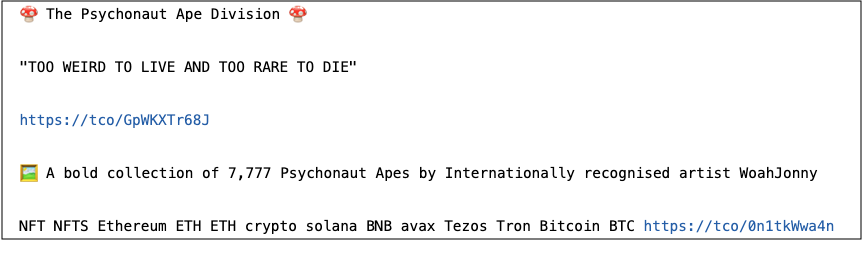
\includegraphics[scale=0.48]{CHAPTER_5/raw_tweet_example.png}
    \caption{Example of raw tweet scraped using the tweepy package through Python}
    \label{raw_tweet_example}
  \end{figure}
\noindent The number of tweets at the end of each hour was continuous and had no major issues from the API response.
\begin{figure}[H]
   \centering
   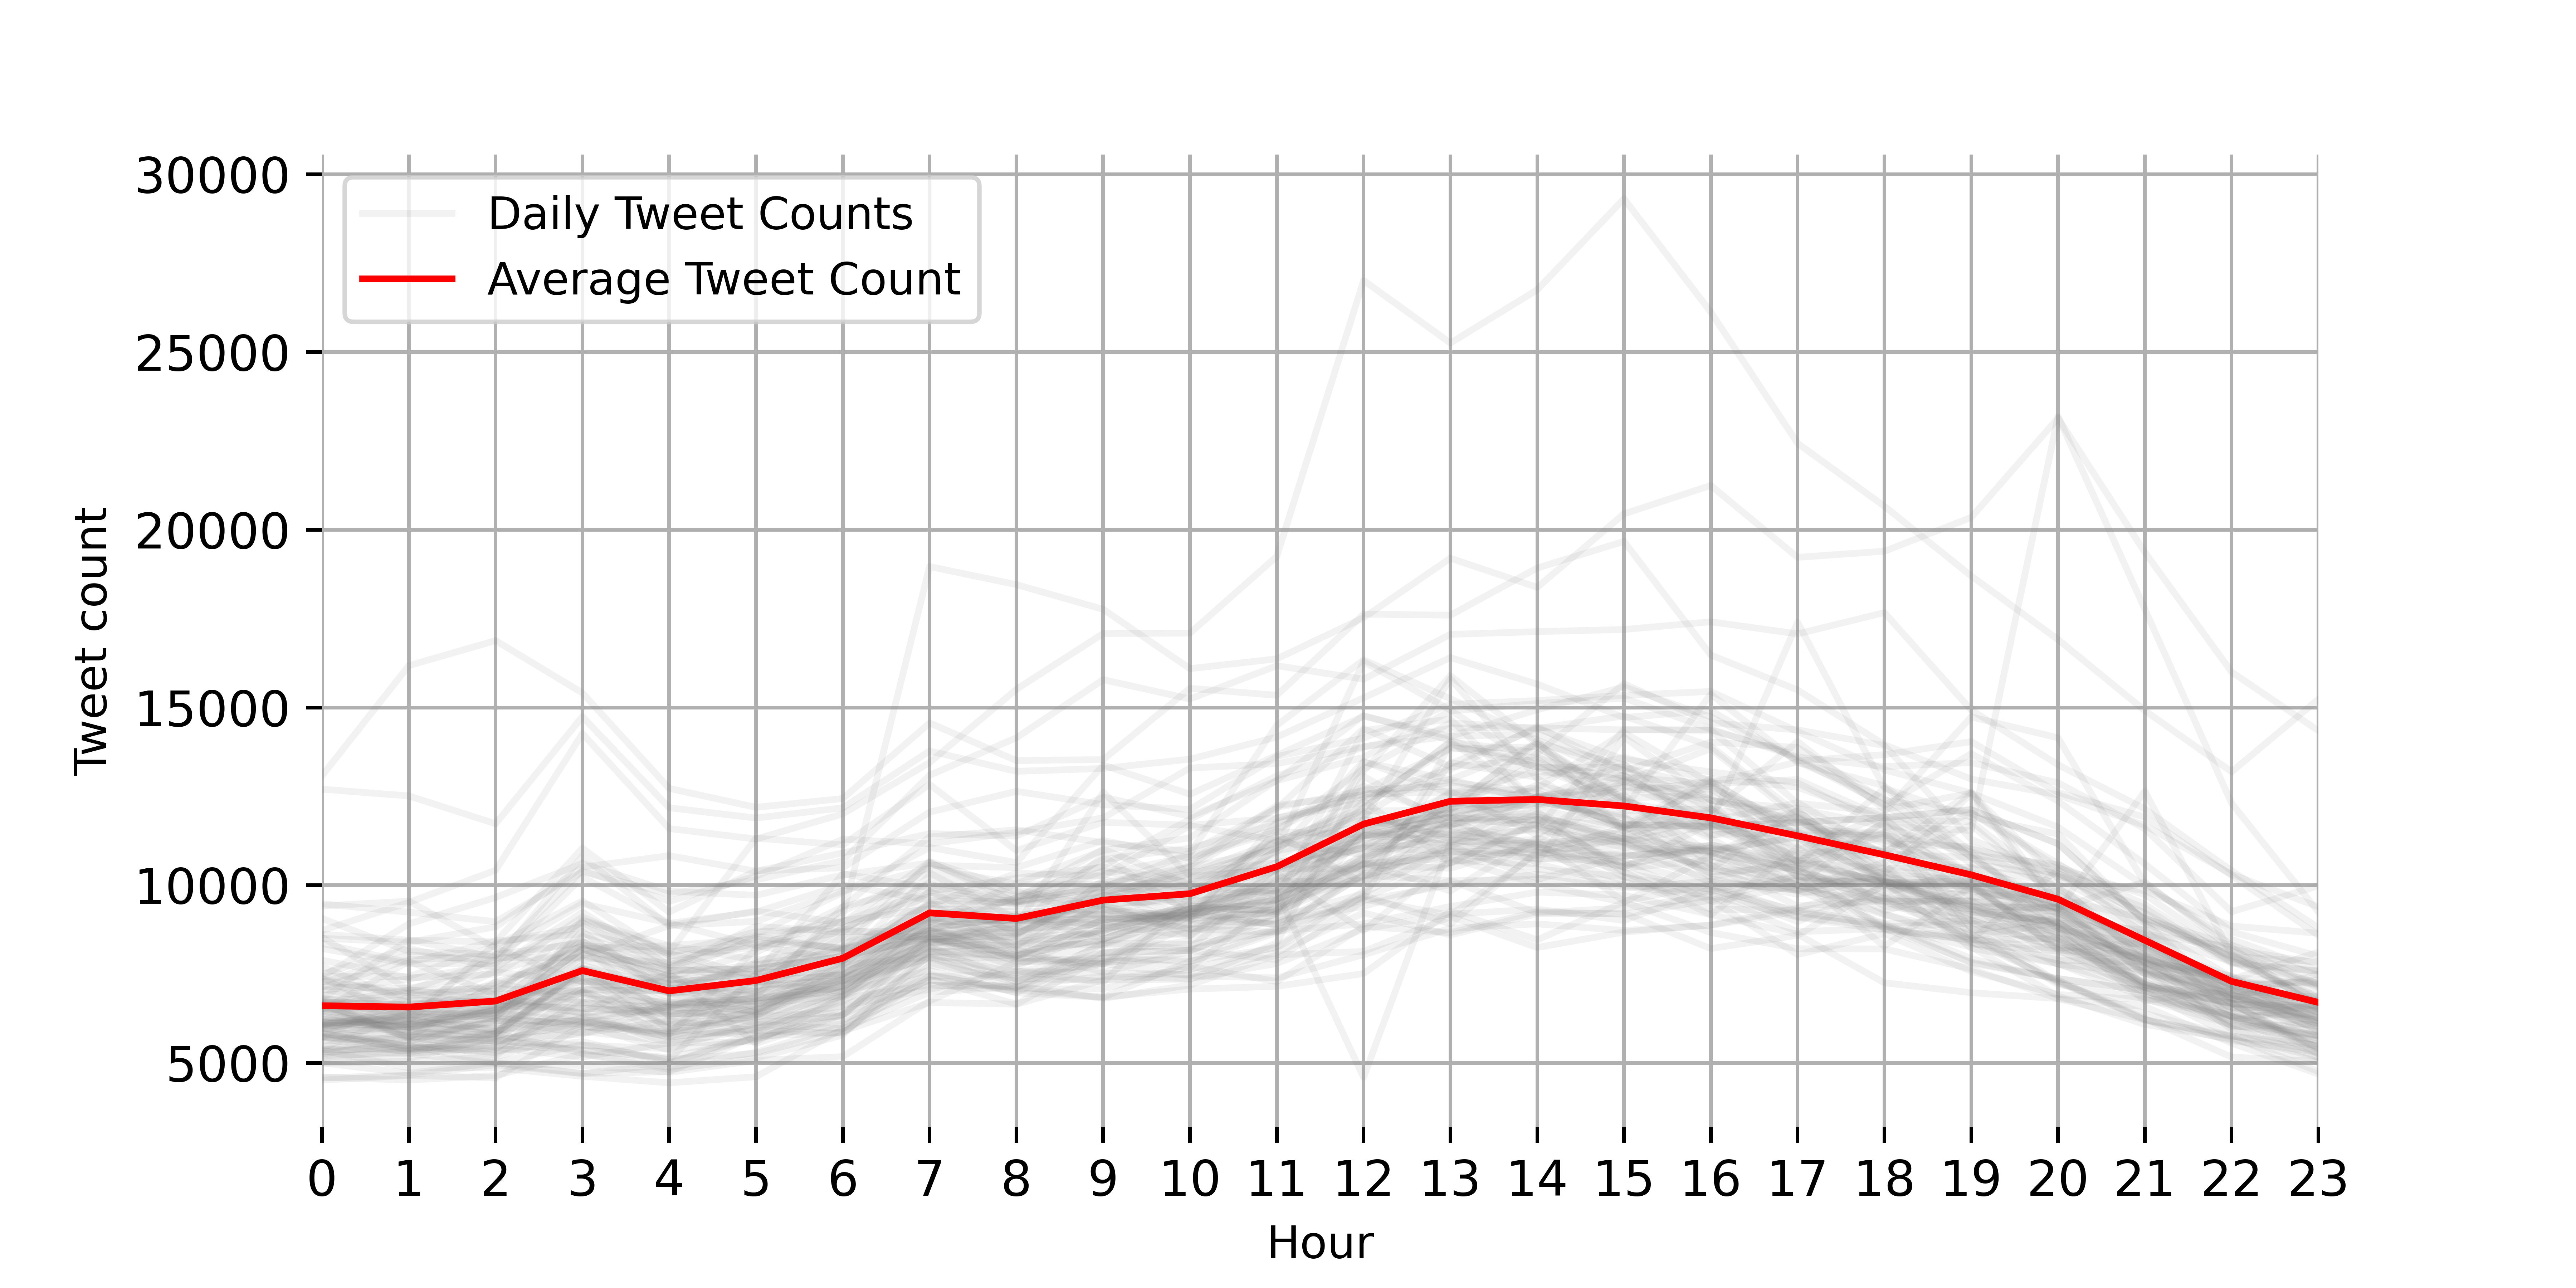
\includegraphics[scale=0.70]{CHAPTER_5/tweet_count_python.png}
   \caption{Distribution of tweet count over each day at the end of every hour over 24 hours}
   \label{tweet_count}
\end{figure}
\noindent The data for the open, high, low, and close prices scrapped from Yahoo Finance was clean and had no issues. However, we did see that not all closing hours have the associated volume. Thus, volume was not included in the final dataset.
\begin{figure}[H]
    \centering
    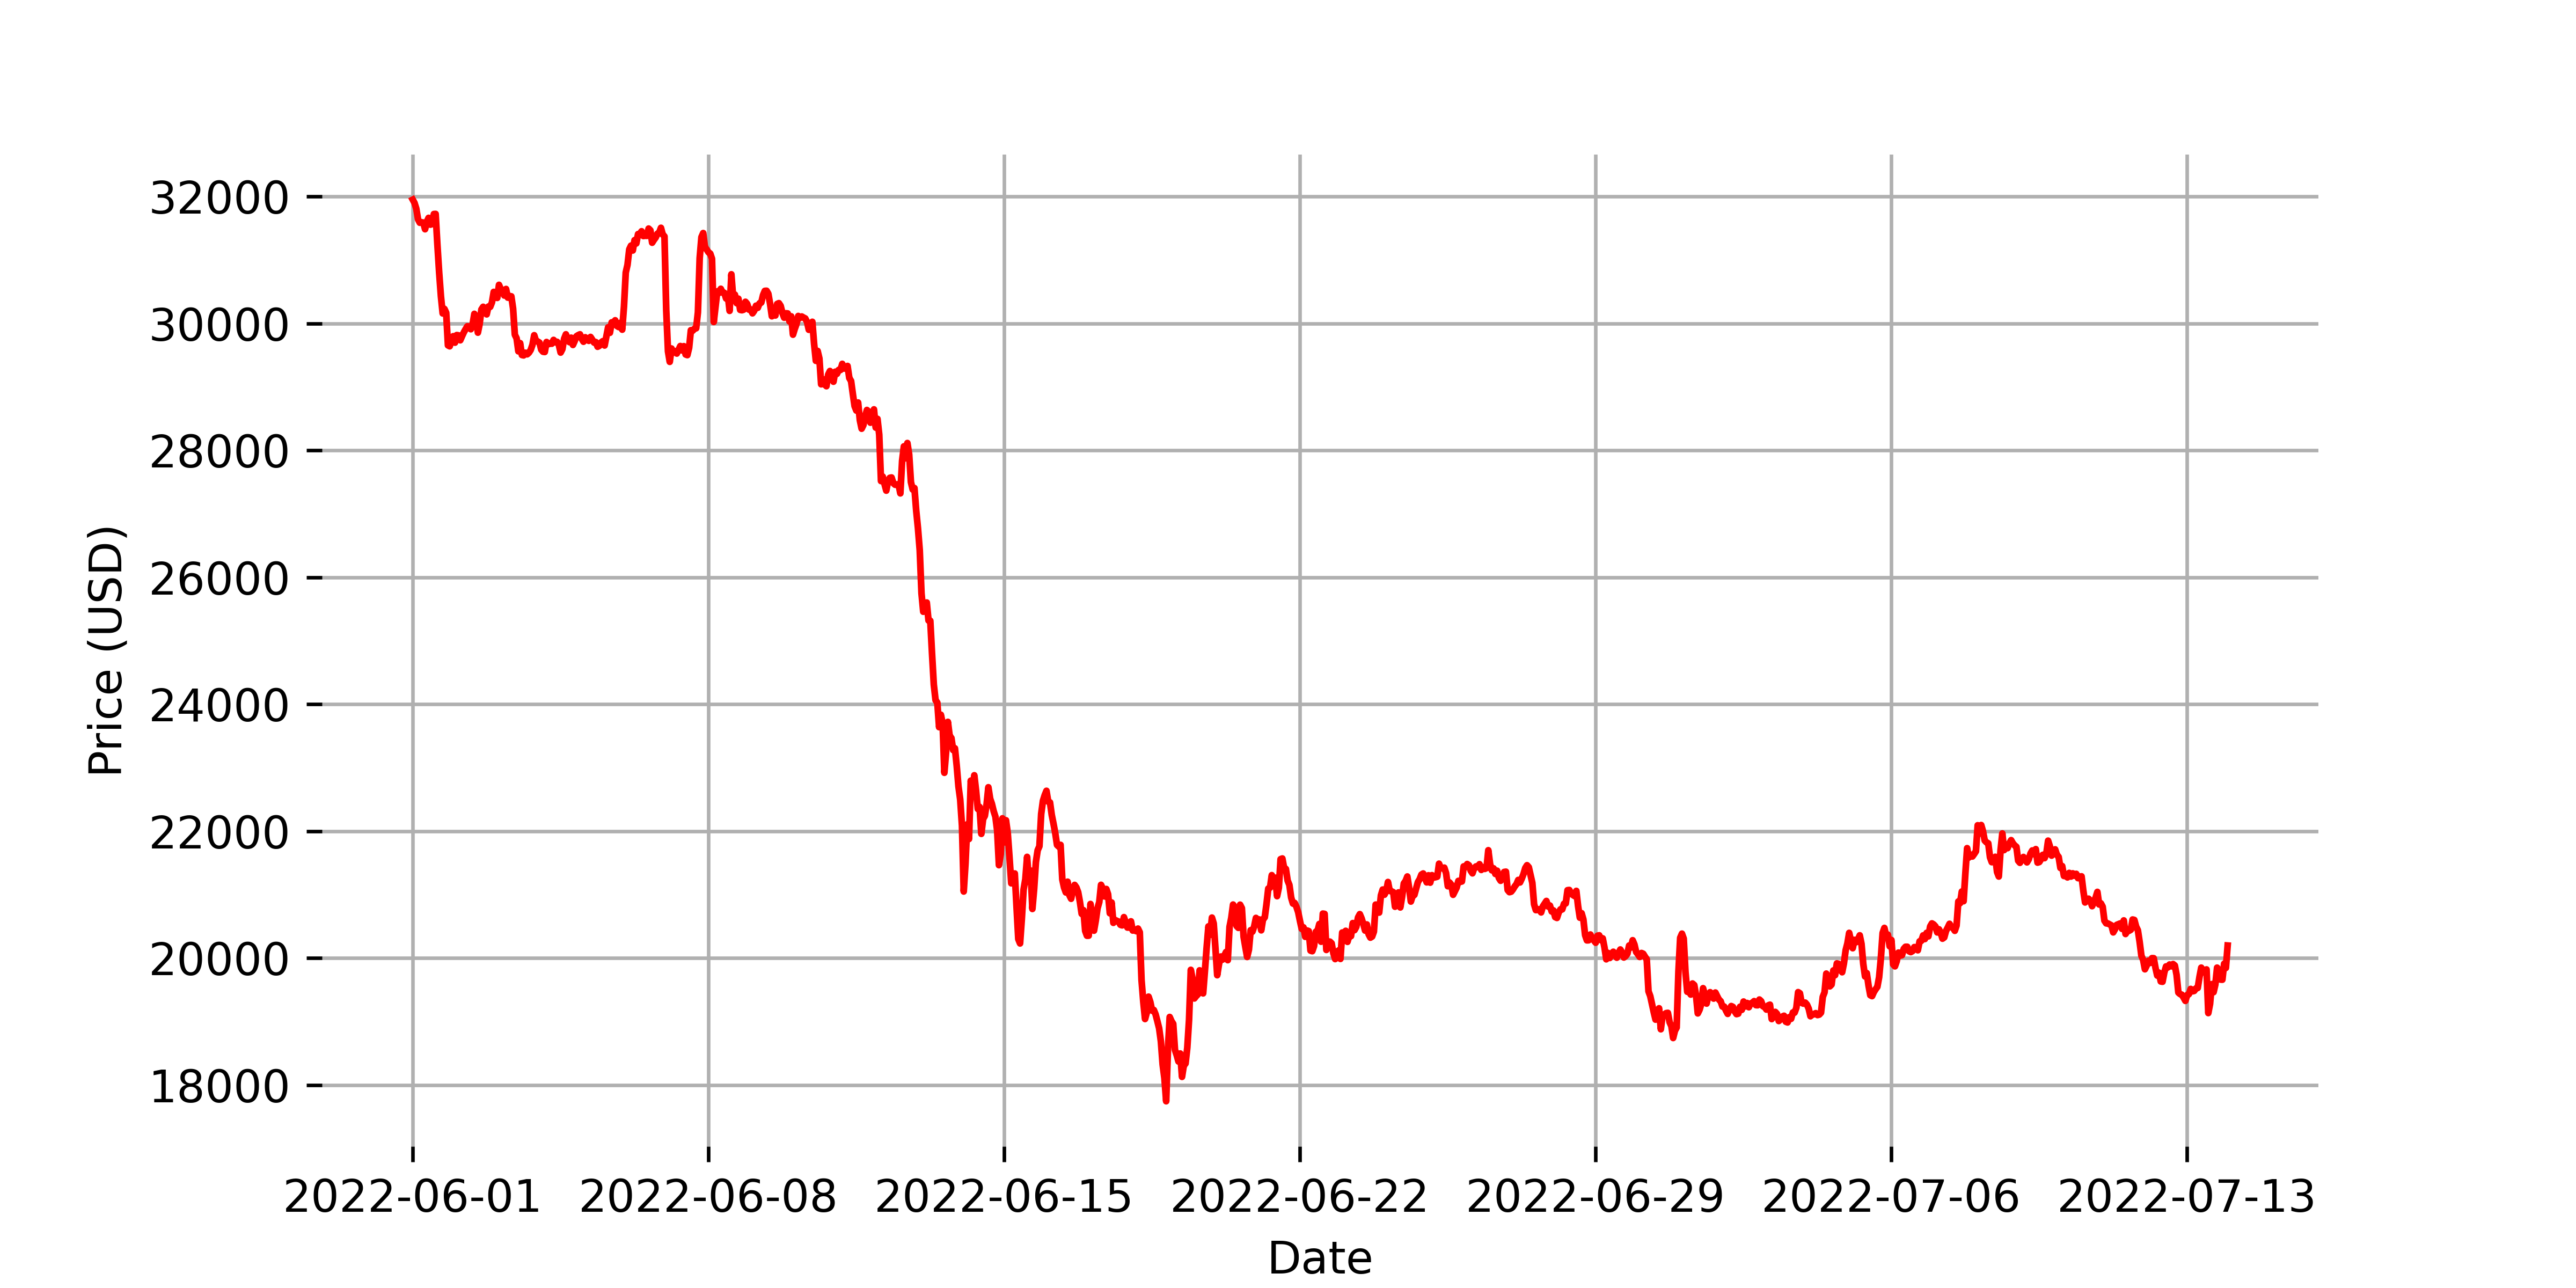
\includegraphics[scale=0.73]{CHAPTER_5/bitcoin_price_python.png}
    \caption{Bitcoin closing price over every hour for everyday}
    \label{bitcoin_price}
 \end{figure}
\section{Feature Engineering}
Feature engineering is the manipulation of our dataset to provide extra features to input in our model to improve accuracy. Manipulation includes addition, deletion, combination and transformation of the dataset. Practical feature engineering is dependent on the business problem and our objective. Common types of feature engineering include scaling and transformation, fitting missing values, feature coding, feature construction and feature extraction. 
\subsection*{Sentiment Analysis on Tweet Data}
In order to be able to quantify the tweets as features in our model, we transform the tweets into numerical values by performing sentiment analysis on them. However, as seen in the tweet example in listing (\ref{raw_tweet_example}), the raw tweet would be difficult for the existing natural language processing model to transform them. Using regular expression syntax in Python, we cleaned the tweets first.
\begin{lstlisting}[language=Python, caption= {Python function to clean Tweets using RegEx (regular expression)}, label= regex_function]
    def pre_process_tweet (text):
    #Remove all links starting with http...
    text = re.sub('https?:\/\/.*[\r\n]*','',text)
    #Remove RT
    text = re.sub('^RT[\s]+','',text)
    #Remove @[User]
    text = re.sub('@[^ ]+', '', text)
    #Remove Punctuation first
    text = text.translate(str.maketrans('','', string.punctuation))
    #Convert text to lower case
    text = text.lower()
    #Remove new line
    text = re.sub('\n',' ',text)
    #Replace emojis with description
    text = demoji.replace_with_desc(text,sep=' ')
    #Reducing whitespaces to one everywhere
    text = re.sub('\s+',' ',text)
    return text
\end{lstlisting}
Applying the python function defined in listing \ref{regex_function} to the raw tweet in \ref{raw_tweet_example} leads to the following string:
\begin{align}
    \label{preprocess_tweet}
    \nonumber
    &\text{'mushroom the psychonaut ape division mushroom too weird to live and too } \\
    \nonumber
    &\text{rare to die framed picture a bold collection of psychonaut apes by  }\\
    \nonumber
    &\text{internationally recognised artist woahjonny nft nfts ethereum eth eth crypto }\\
    &\text{solana bnb avax tezos tron bitcoin btc'}
\end{align}
We apply the pre-process tweet function across the 814,818 tweets that were scraped. Thus, making the tweets easier to process in sentiment analysis models. Once the tweets are clean, we use the RoBERTa model defined in Section \ref{section: transformers} to perform sentiment analysis. We used the version \textit{cardiffnlp/twitter-roberta-base-sentiment} which is made available Hugging Face. 'Twitter-roBERTa-base' for Sentiment Analysis is a pretrained  on approximately 58 million tweets and fine-tuned for sentiment analysis \cite{France2020}. The output of the model are is the percentage of a tweet being negative, neural and positive.
\begin{lstlisting}[language=Python, caption= {Applying the twitter-roberta-base-sentiment model to the preprocessed tweet in (\ref{preprocess_tweet})}, label= roberta_example]
    encoded_text = tokenizer(preprocessed_tweet, return_tensors='pt')
    output = model(**encoded_text)
    scores = output[0][0].detach().numpy()
    scores = softmax(scores)
    scores_dict = {'roberta_neg':scores[0], 'roberta_neu':scores[1], 'roberta_pos':scores[2]}
    print(scores_dict)

>> {'roberta_neg':0.298603, 'roberta_neu':0.5974009, 'roberta_pos':0.10399604}
\end{lstlisting}
We apply the same function through the whole preprocessed dataset to get the scraped tweets' scores. Tweets that were too long or had unknown characters that the model could not process were dropped (less than 0.5\% of the tweet dataset). 
\subsection*{Hourly Averaging}
Processing the point data of all the scrapped tweets can be overly demanding in terms of computational power. This will result to an overfitting and not being able the model the general trend of a single day. Additionally, we do not have point data for price and google trends search index. To overcome this problem, we aggregated the sentiment scores (POS, NEU, NEG) over each hour across the time period. The resulting dataset was $1032 \times 3$ (24 hours for 43 days).

\subsection*{Data Encoding}
%%Influencer Daily Averaging using KMeans Neighbouring
%%Test the difference in average on Daily Basis
\section{Modelling Bitcoin Price using LSTM NN}
\subsection*{Model Architecture and Hyperparameters}
%No Influencer
%With Influencer
%Comparison
\section{Modelling Bitcoin Upticks using Feedforward NN}
\subsection*{Model Architecture and Hyperparameters}
%No Influencer
%With Influencer
%Comparison